\documentclass[tikz]{standalone} 



\usepackage{tikz} 


\usetikzlibrary{arrows.meta}
\usetikzlibrary{patterns}
%\usetikzlibrary{backgrounds}
%\usetikzlibrary{shadows.blur}
\usepackage{xcolor}
\definecolor{myorange}{HTML}{FFA82E}  
\definecolor{myorange2}{HTML}{FFBB5C} 
\definecolor{myorange3}{HTML}{FFCE8A} 
\definecolor{background}{HTML}{FFE1B8}
\definecolor{gray}{HTML}{ADADAD}
\definecolor{gray2}{HTML}{969696}
\definecolor{darkgray}{HTML}{696969}
\definecolor{darkgray2}{HTML}{525252}
\definecolor{dark}{HTML}{3B3B3B}

\begin{document} 

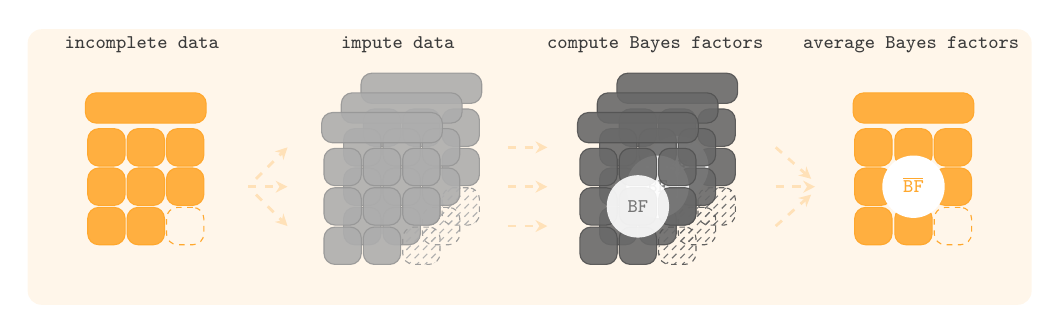
\begin{tikzpicture} 

%background color
\fill[background!30, rounded corners=5pt] (-0.5,0.5) rectangle (12.25,4);

%node stiles
\tikzset{
    neuron3/.style={
        opacity=0.9,
        text opacity=0,
        draw opacity=0.9,
        rounded corners=1pt,
        fill=darkgray,
        text=darkgray
    }
}

\tikzset{
    neuron2/.style={
        opacity=0.9,
        text opacity=0,
        draw opacity=0.9,
        rounded corners=1pt,
        fill=gray,
        text=gray
    }
}

\tikzset{
    neuron/.style={
        opacity=0.9,
        text opacity=0,
        draw opacity=1,
        rounded corners=1pt
    }
}

%left main matrix:
% header
\node[neuron,draw=myorange,fill=myorange,text=myorange,
    text width=1.3cm,text height=0.15cm,
    rounded corners,text centered] at (1,3) {.};

% row 1
\foreach \x in {0.5,1,1.5}{
    \node[neuron,draw=myorange,fill=myorange,text=myorange,
        text width=0.24cm,text height=0.24cm,
        rounded corners,text centered] at (\x,2.5) {.};
}

% row 2
\foreach \x in {0.5,1,1.5}{
    \node[neuron,draw=myorange,fill=myorange,text=myorange,
        text width=0.24cm,text height=0.24cm,
        rounded corners,text centered] at (\x,2) {.};
}

% row 3
\foreach \x in {0.5,1}{
    \node[neuron,draw=myorange,fill=myorange,text=myorange,
        text width=0.24cm,text height=0.24cm,
        rounded corners,text centered] at (\x,1.5) {.};
}

\node[neuron,draw=myorange,draw opacity=1,
    dash pattern=on 2pt off 2pt,
    fill=background!30,text=background!30,
    text width=0.24cm,text height=0.24cm,
    rounded corners,text centered] at (1.5,1.5) {.};

%left secondary matrices: upper, middle and lower


% header
\node[neuron2,draw=gray2,
    text width=1.3cm,text height=0.15cm,
    rounded corners,text centered] at (4.5,3.25) {.};

% row 1
\foreach \x in {4,4.5,5}{
    \node[neuron2,draw=gray2,
        text width=0.24cm,text height=0.24cm,
        rounded corners,text centered] at (\x,2.75) {.};
}

% row 2
\foreach \x in {4,4.5,5}{
    \node[neuron2,draw=gray2,
        text width=0.24cm,text height=0.24cm,
        rounded corners,text centered] at (\x,2.25) {.};
}

% row 3
\foreach \x in {4,4.5}{
    \node[neuron2,draw=gray2,
        text width=0.24cm,text height=0.24cm,
        rounded corners,text centered] at (\x,1.75) {.};
}

\node[neuron2,draw=gray2,draw opacity=0.9,
    dash pattern=on 2pt off 2pt,
    pattern=north east lines,
    pattern color=gray,
    %fill=background!30,
    text=background!30,
    text width=0.24cm,text height=0.24cm,
    rounded corners,text centered] at (5,1.75) {.};

% header
\node[neuron2,draw=gray2,
    text width=1.3cm,text height=0.15cm,
    rounded corners,text centered] at (4.25,3) {.};

% row 1
\foreach \x in {3.75,4.25,4.75}{
    \node[neuron2,draw=gray2,
        text width=0.24cm,text height=0.24cm,
        rounded corners,text centered] at (\x,2.5) {.};
}

% row 2
\foreach \x in {3.75,4.25,4.75}{
    \node[neuron2,draw=gray2,
        text width=0.24cm,text height=0.24cm,
        rounded corners,text centered] at (\x,2) {.};
}

% row 3
\foreach \x in {3.75,4.25}{
    \node[neuron2,draw=gray2,
        text width=0.24cm,text height=0.24cm,
        rounded corners,text centered] at (\x,1.5) {.};
}

\node[neuron2,draw=gray2,draw opacity=0.9,
    dash pattern=on 2pt off 2pt,
    pattern=north east lines,
    pattern color=gray,
    %fill=background!30,
    text=background!30,
    text width=0.24cm,text height=0.24cm,
    rounded corners,text centered] at (4.75,1.5) {.};


% header
\node[neuron2,draw=gray2,
    text width=1.3cm,text height=0.15cm,
    rounded corners,text centered] at (4,2.75) {.};

% row 1
\foreach \x in {3.5,4,4.5}{
    \node[neuron2,draw=gray2,
        text width=0.24cm,text height=0.24cm,
        rounded corners,text centered] at (\x,2.25) {.};
}

% row 2
\foreach \x in {3.5,4,4.5}{
    \node[neuron2,draw=gray2,
        text width=0.24cm,text height=0.24cm,
        rounded corners,text centered] at (\x,1.75) {.};
}

% row 3
\foreach \x in {3.5,4}{
    \node[neuron2,draw=gray2,
        text width=0.24cm,text height=0.24cm,
        rounded corners,text centered] at (\x,1.25) {.};
}

\node[neuron2,draw=gray2,draw opacity=0.9,
    dash pattern=on 2pt off 2pt,
    pattern=north east lines,
    pattern color=gray,
    %fill=background!30,
    text=background!30,
    text width=0.24cm,text height=0.24cm,
    rounded corners,text centered] at (4.5,1.25) {.};
    
%right secondary matrices: upper, middle and lower
% header
\node[neuron3,draw=darkgray2,
    text width=1.3cm,text height=0.15cm,
    rounded corners,text centered] at (7.75,3.25) {.};

% row 1
\foreach \x in {7.25,7.75,8.25}{
    \node[neuron3,draw=darkgray2,
        text width=0.24cm,text height=0.24cm,
        rounded corners,text centered] at (\x,2.75) {.};
}

% row 2
\foreach \x in {7.25,7.75,8.25}{
    \node[neuron3,draw=darkgray2,
        text width=0.24cm,text height=0.24cm,
        rounded corners,text centered] at (\x,2.25) {.};
}

% row 3
\foreach \x in {7.25,7.75}{
    \node[neuron3,draw=darkgray2,
        text width=0.24cm,text height=0.24cm,
        rounded corners,text centered] at (\x,1.75) {.};
}

\node[neuron3,draw=darkgray2,draw opacity=0.9,
    dash pattern=on 2pt off 2pt,
    pattern=north east lines,
    pattern color=darkgray,
    %fill=background!30,
    text=background!30,
    text width=0.24cm,text height=0.24cm,
    rounded corners,text centered] at (8.25,1.75) {.};

\node[
    circle,
    fill=white,
    draw=none,
    text=darkgray,
    opacity = 0.9,
    font=\scriptsize\bfseries\ttfamily,
    inner sep=5pt
] at (7.75,2.25) {BF};

% header
\node[neuron3,draw=darkgray2,
    text width=1.3cm,text height=0.15cm,
    rounded corners,text centered] at (7.5,3) {.};

% row 1
\foreach \x in {7,7.5,8}{
    \node[neuron3,draw=darkgray2,
        text width=0.24cm,text height=0.24cm,
        rounded corners,text centered] at (\x,2.5) {.};
}

% row 2
\foreach \x in {7,7.5,8}{
    \node[neuron3,draw=darkgray2,
        text width=0.24cm,text height=0.24cm,
        rounded corners,text centered] at (\x,2) {.};
}

% row 3
\foreach \x in {7,7.5}{
    \node[neuron3,draw=darkgray2,
        text width=0.24cm,text height=0.24cm,
        rounded corners,text centered] at (\x,1.5) {.};
}

\node[neuron3,draw=darkgray2,draw opacity=0.9,
    dash pattern=on 2pt off 2pt,
    pattern=north east lines,
    pattern color=darkgray,
    %fill=background!30,
    text=background!30,
    text width=0.24cm,text height=0.24cm,
    rounded corners,text centered] at (8,1.5) {.};

\node[
    circle,
    fill=white,
    draw=none,
    text=darkgray,
    opacity = 0.9,
    font=\scriptsize\bfseries\ttfamily,
    inner sep=5pt
] at (7.5,2) {BF};

% header
\node[neuron3,draw=darkgray2,
    text width=1.3cm,text height=0.15cm,
    rounded corners,text centered] at (7.25,2.75) {.};

% row 1
\foreach \x in {6.75,7.25,7.75}{
    \node[neuron3,draw=darkgray2,
        text width=0.24cm,text height=0.24cm,
        rounded corners,text centered] at (\x,2.25) {.};
}

% row 2
\foreach \x in {6.75,7.25,7.75}{
    \node[neuron3,draw=darkgray2,
        text width=0.24cm,text height=0.24cm,
        rounded corners,text centered] at (\x,1.75) {.};
}

% row 3
\foreach \x in {6.75,7.25}{
    \node[neuron3,draw=darkgray2,
        text width=0.24cm,text height=0.24cm,
        rounded corners,text centered] at (\x,1.25) {.};
}

\node[neuron3,draw=darkgray2,draw opacity=0.9,
    dash pattern=on 2pt off 2pt,
    pattern=north east lines,
    pattern color=darkgray,
    %fill=background!30,
    text=background!30,
    text width=0.24cm,text height=0.24cm,
    rounded corners,text centered] at (7.75,1.25) {.};

\node[
    circle,
    fill=white,
    draw=none,
    text=darkgray,
    opacity = 0.9,
    font=\scriptsize\bfseries\ttfamily,
    inner sep=5pt
] at (7.25,1.75) {BF};

%right main matrix:
% header
\node[neuron,draw=myorange,fill=myorange,text=myorange,
    text width=1.3cm,text height=0.15cm,
    rounded corners,text centered] at (10.75,3) {.};

% row 1
\foreach \x in {10.24,10.75,11.25}{
    \node[neuron,draw=myorange,fill=myorange,text=myorange,
        text width=0.24cm,text height=0.24cm,
        rounded corners,text centered] at (\x,2.5) {.};
}

% row 2
\foreach \x in {10.24,10.75,11.25}{
    \node[neuron,draw=myorange,fill=myorange,text=myorange,
        text width=0.24cm,text height=0.24cm,
        rounded corners,text centered] at (\x,2) {.};
}

% row 3
\foreach \x in {10.24,10.75}{
    \node[neuron,draw=myorange,fill=myorange,text=myorange,
        text width=0.24cm,text height=0.24cm,
        rounded corners,text centered] at (\x,1.5) {.};
}

\node[neuron,draw=myorange,draw opacity=1,
    dash pattern=on 2pt off 2pt,
    fill=background!30,text=background!30,
    text width=0.24cm,text height=0.24cm,
    rounded corners,text centered] at (11.25,1.5) {.};

\node[
    circle,
    fill=white,
    draw=none,
    text=myorange,
    font=\scriptsize\bfseries\ttfamily,
    inner sep=5pt
] at (10.75,2) {BF};

%Write text
%overline last BF
%\node[text=myorange, font=\Large\ttfamily] at (10.75,2.1) {-};
\draw[myorange, line width=0.4pt]
    (10.62,2.1) -- (10.87,2.1);

%upper text
\node[text=dark, font=\scriptsize\bfseries\ttfamily] at (0.95,3.8) {incomplete data};

\node[text=dark, font=\scriptsize\bfseries\ttfamily] at (4.2,3.8) {impute data};

\node[text=dark, font=\scriptsize\bfseries\ttfamily] at (7.47,3.8) {compute Bayes factors};

\node[text=dark, font=\scriptsize\bfseries\ttfamily] at (10.72,3.8) {average Bayes factors};

%arrows:
\draw[ -{Stealth[length=1.5mm,width=1.5mm]}, draw=background, dashed , line width=1pt] (2.3,2) to
%[out=-20,in=80] 
(2.8,2);
\draw[ -{Stealth[length=1.5mm,width=1.5mm]}, draw=background, dashed , line width=1pt] (2.4,2.1) to
%[out=-20,in=80] 
(2.8,2.5);
\draw[ -{Stealth[length=1.5mm,width=1.5mm]}, draw=background, dashed , line width=1pt] (2.4,1.9) to
%[out=-20,in=80] 
(2.8,1.5);

\draw[ -{Stealth[length=1.5mm,width=1.5mm]}, draw=background, dashed , line width=1pt] (5.6,2) to
%[out=-20,in=80] 
(6.1,2);
\draw[ -{Stealth[length=1.5mm,width=1.5mm]}, draw=background, dashed , line width=1pt] (5.6,2.5) to
%[out=-20,in=80] 
(6.1,2.5);
\draw[ -{Stealth[length=1.5mm,width=1.5mm]}, draw=background, dashed , line width=1pt] (5.6,1.5) to
%[out=-20,in=80] 
(6.1,1.5);

\draw[ -{Stealth[length=1.5mm,width=1.5mm]}, draw=background, dashed , line width=1pt] (9,2) to
%[out=-20,in=80] 
(9.5,2);
\draw[ -{Stealth[length=1.5mm,width=1.5mm]}, draw=background, dashed , line width=1pt] (9,2.5) to
%[out=-20,in=80] 
(9.45,2.1);
\draw[ -{Stealth[length=1.5mm,width=1.5mm]}, draw=background, dashed , line width=1pt] (9,1.5) to
%[out=-20,in=80] 
(9.45,1.9);

\end{tikzpicture} 

\end{document}
